\section{Overview of Future Research}
%All DNA-templated processes in the nucleus occur in the context of the local chromatin environment.  
My research program has been focused on understanding how chromatin shapes the DNA replication program in \scer and \dros. We have taken advantage of the unique features and strengths of each organism -- well defined cis-acting and chromatin determinants of origin function in \scer and the more complex epigenetic features that regulate origin selection and activation in \dros.  
We will continue to use the strengths of each model system to address fundamental questions regarding the inheritance of genetic and epigenetic information. We are also excited to extend our nucleotide resolution GCOPs to investigate chromatin dynamics associated with DNA damage and repair. Finally, in collaboration with Alex Hartemink (Computer Science, Duke) and Greg Crawford (Pediatrics, Duke) we have recently been awarded a collaborative NIGMS R01 to probe chromatin-based mechanisms inside the `black box' of transcriptional regulation. 

\sheading{DNA Replication}
\ssheading{Chromatin dynamics during initiation of DNA replication in \scer}
%Beginning in G1, a series of tightly orchestrated biochemical events occur at each origin of DNA replication ultimately leading up to initiation of DNA replication in S-phase\citep{}.  
How does the local chromatin environment, which is unique to each origin, modulate ORC binding, pre-RC assembly, and initiation?  We have already identified a series of specific nucleosome remodeling events that occur during ORC binding (G2) and pre-RC assembly (G1)\citep{Eaton2010-iy,Belsky2015-li} which are correlated with origin efficiency\citep{Belsky2015-li}. We now propose to examine changes in chromatin structure that are associated with the assembly of the pre-initiation complex and priming of DNA replication.  We hypothesize that the steps leading up to unwinding of the DNA and the transition of the Mcm2-7 complex from encircling dsDNA to ssDNA will result in the specific eviction or sliding of origin flanking nucleosomes.  We also expect that local chromatin features unique to each origin (\eg flanking DNA binding factors and local transcription) will contribute to the symmetry and extent of nucleosome remodeling and eviction.  We will use conditional  mutants (ts, degron, anchor away\citep{Haruki2008-qe} or combinations) of key initiation factors (\eg primase or \textit{Mcm10}) to block DNA replication immediately prior to initiation.  Alternatively, we will attempt to block initiation using the conditional expression of MCM mutants (MCM3RA) defective for initiation but not Cdc45 and GINS loading \invitro\citep{Kang2014-iu}. While the GCOP mapping will provide a factor agnostic assessment of origin chromatin architecture, we will also use ChIP-exo\citep{Rhee2011-yi} to probe the location and identity of specific structural footprints observed in the GCOPs.  We expect to identify and decipher the key changes in chromatin structure that accompany the transition of the pre-RC into the pre-IC and ultimately into a functional bidirectional replisome.  
%\ssheading{Mcm2-7 loading is limited by chromatin architecture}
\begin{floatingfigure}[r]{2.1in}
\vspace{-8mm}
\begin{center}
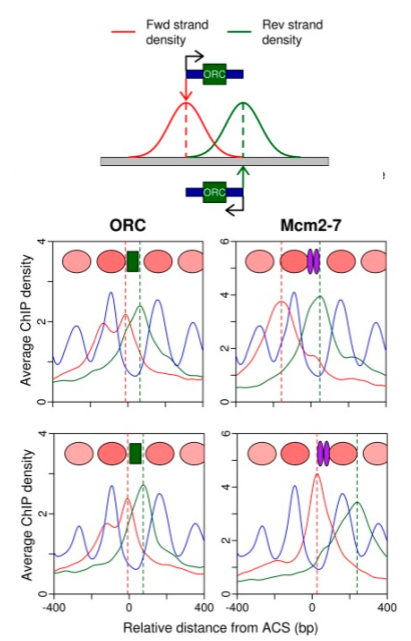
\includegraphics[width=2.1in]{r35_figures/mcm_histone.png}
\end{center}
\vspace{3mm}
\caption{Asymmetric Mcm2-7 loading at replication origins.  The ends of ChIP fragments were analyzed to precisely localize ORC and MCM2-7.  ORC resolves to the ACS and exhibts an interaction with the leftmost flanking nucleosome.  Mcm2-7 localizes up or downstream of the ACS and is in complex with the up or downstream flanking nucleosome.}%
\end{floatingfigure}%


Bi-directional DNA replication emanating from an origin is an inherently symmetrical event.  Despite this symmetry, there is striking asymmetry in a number of origin features.  For example, the T-rich ACS and downstream A-rich region is a polar sequence that is asymmetrically located between two flanking nucleosomes. Further, we have demonstrated that the loading of double hexamer of Mcm2-7 occurs either up or downstream from the oriented ACS and is tightly coupled with the flanking nucleosome ({\color{dukeblue}\textbf{Figure 3}}) \citep{Belsky2015-li}. We will identify the mechanism(s) by which Mcm2-7 loading is asymmetric, coupled with a flanking nucleosome, and limited to one double hexamer per origin.  Although the significance of why each origin adopts a specific Mcm2-7 loading configuration (up or downstream of the ACS) is currently unclear, it is reasonable to speculate that specific configurations may facilitate initiation and origin efficiency -- especially in the context of other surrounding chromatin features such as histone modifications, direction of transcription and nucleosome turn-over.  We will first test the role of known and conserved mutants that disrupt the interaction between Mcm2 and histone H3\citep{Huang2015-fk,Foltman2013-dk}.  While these Mcm2 mutations do not exhibit a gross defect in transit through S-phase, they are thought to impair chromatin assembly and disassembly at the fork\citep{Foltman2013-dk}.  If we observe that interaction with the origin flanking nucleosome is disrupted or there is loss of polarity in Mcm2-7 loading, we will carefully assess replication timing and the kinetics of initiation \invivo.  Alternative approaches will include a proteomic based approach to identify potential histone modifications that are enriched on nucleosomes immunoprecipiated with the Mcm2-7 complex (LoS Mosely), and disrupting transcription of origin flanking genes to prevent transcription into the origin which may influence the polarity of origin loading\citep{Gros2015-oo}.  Importantly, does elimination of any of these mechanisms result in the loading of additional Mcm2-7 double hexamers per origin or perturbations in origin efficiency? Finally, we will continue to collaborate with the Bell laboratory in order to confirm and further dissect our \invivo findings in a reconstituted system (LoS Bell).  

\ssheading{Origin selection and activation in \dros}
Despite the conservation of replication initiation factors, identifying the precise locations where DNA replication starts in higher eukaryotes has been a long standing and controversial question\citep{Prioleau2016-bj}. The canonical model is that ORC recruits the Mcm2-7 helicase to specific locations in the genome to function as origins in the next S-phase. Although ORC does map to specific sites in the genome\citep{Miotto2016-jt}, initiation of DNA replication is not confined to specific locations but instead maps to broad zones of initiation ($>$30 kb)\citep{Petryk2016-rr}. We propose that initiation in higher eukaryotes is dependent not on the localization of ORC, but rather the genome-wide distribution of the Mcm2-7 complex. This model is supported by our recent work demonstrating that the distribution of the Mcm2-7 complex as \dros cells enter S-phase is not associated with ORC, but rather distributed throughout the genome and shaped by transcription\citep{Powell2015-af}.  These data are also supported by \invitro and \invivo studies in yeast where the precise location of the Mcm2-7 complex can be displaced for short distances away from the origin by active transcription\citep{Gros2015-oo}.  

The loaded Mcm2-7 complex is capable of translocating on naked DNA -- but how does the complex seemingly redistribute throughout the complex chromatin landscape of a metazoan chromosome?  Three possible models are that the Mcm2-7 complex is able to i) translocate away from the ORC binding site; ii) be loaded at a distance from the ORC binding via DNA looping; iii) load promiscuously throughout the genome in an ORC independent manner\citep{Shibata2016-uc}.  The genomic tools and cell cycle synchronization methods that we developed to examine the CDK-regulated step wise loading of the Mcm2-7 complex in \dros coupled with recent advances in CRISPR/Cas9 methodologies\citep{Kunzelmann2016-sf} have us well positioned to test these models.  For example, while we have shown loading of the full Mcm2-7 complement is dependent on Cdc6 and Cdt1\citep{Powell2015-af}, we can also conditionally remove ORC (using degrons) prior to the second wave of Mcm2-7 loading to test the dependence on ORC.  These and other experiments will provide new insights into how metazoan origins of replication are specified.   

We will continue our ongoing collaboration with the Duronio group at UNC to investigate the role of specific chromatin marks in regulating replication timing, genome stability and origin usage in \dros\citep{Li2016-fi}(LoS Duronio). Using a genetic histone replacement strategy\citep{McKay2015-nn}, we will be able to directly test the impact of specific histone tail mutants on DNA replication in proliferating tissues. %Importanty, this approach provides a direct assesment of the role of specific    %The Duronio group has developed a genetic histone replacement strategy for the fly\citep{McKay2015-nn}, allowing us to directly test the impact of specific histone tail mutants on DNA replication in proliferating tissues (\eg imaginal discs).  Unlike manipulation of chromatin modifying enzymes, this approach eliminates potential off target actions and provides an unbiased assessment of the role of specific chromatin modifications in regulating the DNA replication program.
\begin{floatingfigure}[l]{3.55in}
\vspace{-6mm}
\begin{center}
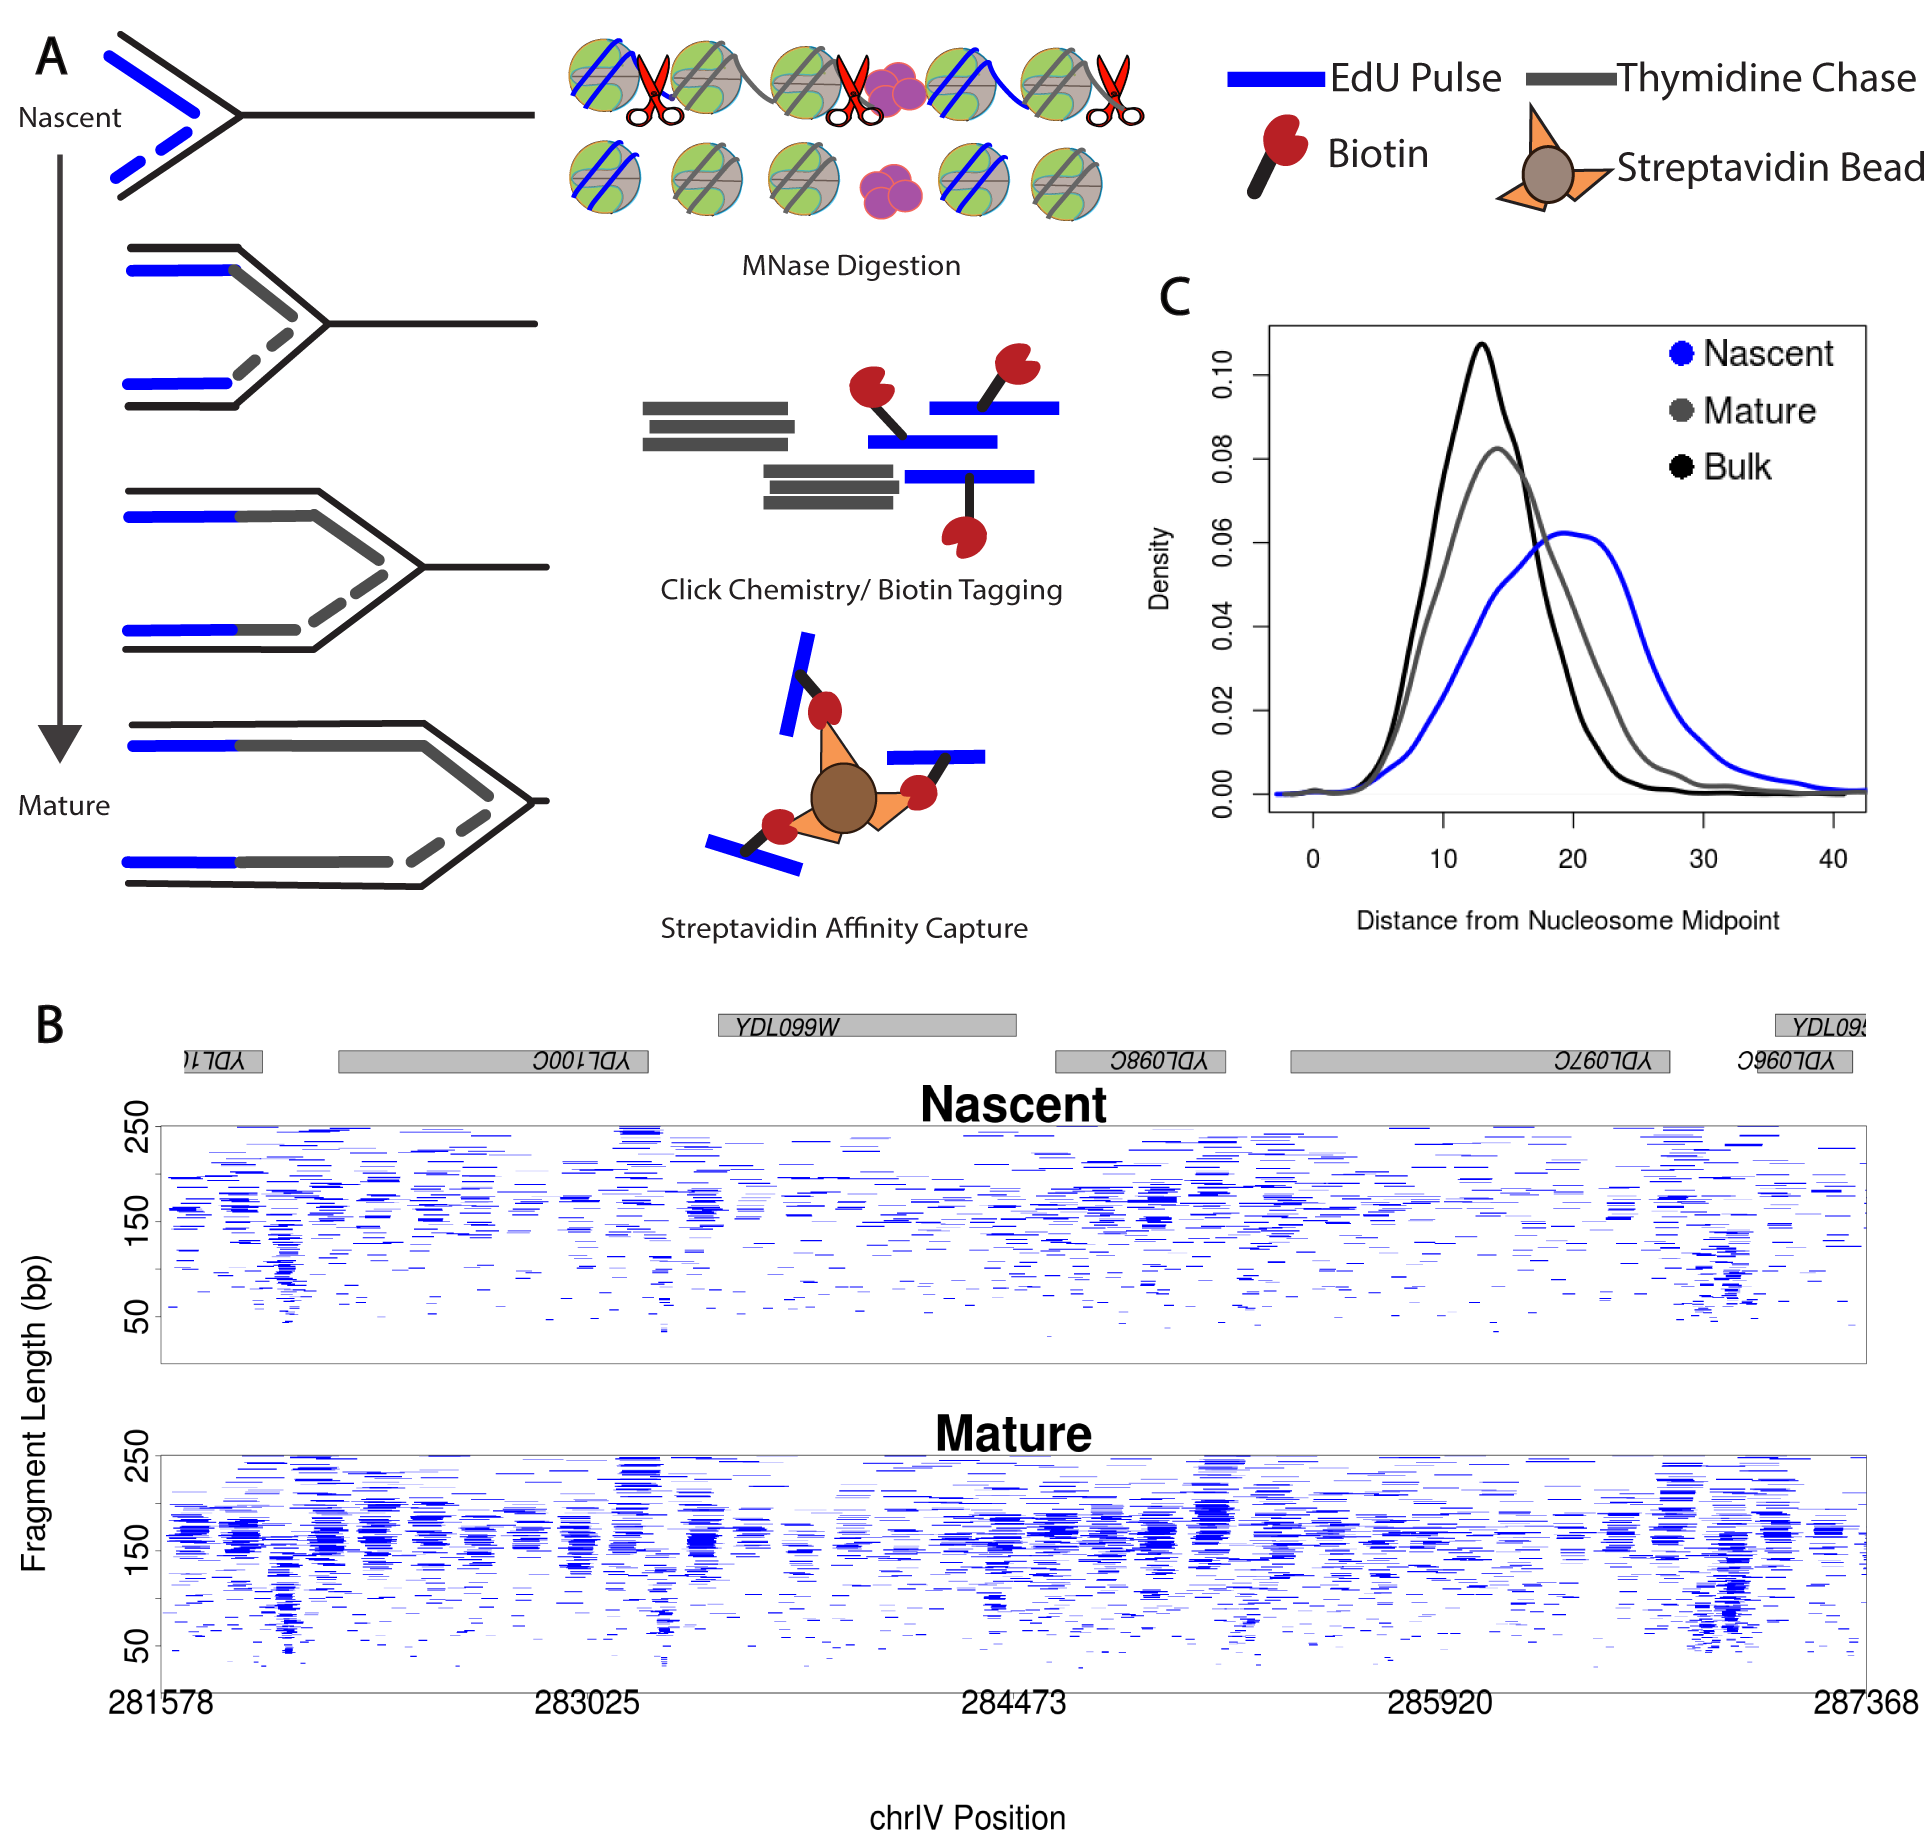
\includegraphics[width=3.55in]{r35_figures/dave_figure2.png}
\end{center}
\vspace{2mm}
\caption{\textbf{A}. Schematic for determining chromatin structure for nascent and maturing chromatin labeled with EdU. \textbf{B}. GCOP of nascent and mature chromatin. \textbf{C}.  Distribution of nucleosome midpoints for bulk (black), mature (gray) and nascent (blue) chromatin demonstrating that nascent chromatin lacks precise nucleosome positioning.}%
\end{floatingfigure}


%\ssheading{Chromatin assembly behind the replication fork}
\ssheading{Role of DNA Replication in Establishing Chromatin Architecture}
%DNA replication plays an integral role in propagating the parental epigenetic state to newly copied sequences.  
DNA replication results in the complete disassembly of chromatin, which must be re-established behind the replication fork in order to propagate the original epigenetic state. Chromatin restoration on nascent DNA is a complex and regulated process, including nucleosome assembly, remodeling, and deposition of histone variants\citep{MacAlpine2013-ds}.  Recently, proteomic techniques have been developed to study the proteins associated with replicative chromatin in a temporal fashion\citep{Alabert2014-io,Sirbu2011-wx}. %Nascent and mature chromatin are differentiated by the incorporation of nucleoside analogs (e.g. BrdU, EdU) followed by the immunoprecipitation of labeled chromatin after a short pulse of only a few minutes for nascent chromatin or followed by a longer chase period for mature chromatin. 
While these approaches focus on studying large pools of proteins associated at multiple phases of replication, they do not provide the spatial or temporal information of chromatin maturation at individual loci. 

We have extended our GCOP assay to profile EdU labeled chromatin in order to examine chromatin occupancy for nascent and mature chromatin ({\color{dukeblue}\textbf{Figure 4}}).  Similar approaches to examine chromatin maturation have very recently been reported in yeast\citep{Vasseur2016-rx} and \dros\citep{Ramachandran2016-zu}; however, these approaches focused on nucleosomes and not the occupancy of smaller DNA binding proteins.  As a proof of principle, we pulse labeled asynchronous cells with Edu for 10 minutes and chased with thymidine for 0 or 40 minutes to recover nascent and mature chromatin, respectively.  Importantly, the  assay monitors the kinetics of chromatin maturation behind the fork. We find significantly less chromatin organization in the nascent chromatin relative to mature chromatin. %Interestingly, we also find locus specific differences in chromatin maturation dependent on origin efficiency.  The chromatin structure at efficient origins matures faster than inefficient origins suggesting there are differences in origin re-assembly between actively firing and passively replicated origins.

We expect to address multiple fundamental questions in chromatin biology. For example, are there locus-specific differences in chromatin maturation? -- perhaps we will identify `epigenetic fragile sites' or locations that are slow to re-establish their chromatin landscape. Is there a difference in replication or transcription dependent chromatin organization? Do all DNA-binding factors re-associate with the chromatin with the same kinetics, or are there factor-specific and locus specific differences?   As this work matures we will interrogate the role of histone chaperones and chromatin remodelers in the re-establishment of chromatin organization behind the replication fork.  

%\newpage
\sheading{DNA Damage}
Elegant genetic and biochemical experiments have elucidated many of the molecular events associated with the recognition and repair of  double-strand breaks\citep{Haber2016-ca,Lieber2010-cl,Renkawitz2014-jz,Jasin2013-fv}.  In addition to the factors required for break recognition, processing and repair via homologous recombination or non-homologous end joining, the local chromatin environment also influences the accessibility of the break site
and the kinetics of recognition and repair\citep{Price2013-lp,Smerdon1991-sv}. Prior studies have noticed a loss of nucleosome occupancy following break recognition by the Mre11-Rad50-Xrs2 (MRX) complex\citep{Tsukuda2005-bm}, which is a conserved phenomena in mammalian cells\citep{Berkovich2007-it,Goldstein2013-kb}. However, these experiments have lacked the temporal and spatial resolution to discern the precise mechanisms by which nucleosome organization and occupancy are lost (\eg eviction or sliding of nucleosomes?) and the fate of bound transcription factors.  We will use our GCOP assay to precisely and quantitatively profile the temporal cascade of chromatin structure changes that occur surrounding site-specific double strand breaks and their subsequent repair via NHEJ or HR. Our investigations into DNA damage and DSB repair will be further augmented by collaboration with Jim Haber at Brandeis (LoS Haber). %In order to interpret our GCOP data in the context of the DNA repair field, we will received guidance and advice from Jim Haber at Brandies (LoS Haber).


\ssheading{Chromatin alterations at site specific DSBs}
%using a donorless
We are able to monitor the specific chromatin changes that occur in response to a GAL::HO induced DSB in the absence of a donor for HR mediated repair.  Proof of principle experiments at an ectopic HO cut site in the \textit{PHO5} locus reveal the asymmetric eviction of a flanking nucleosome, sliding of distal nucleosomes until impeded by a neighboring Fkh2 bound site and the recruitment of a DNA binding factor to the break ({\color{dukeblue}\textbf{Figure 5}}).  Although we can detect a new occupancy footprint at either side of the  break, we do not know the identity of the factor -- it could represent the MRX complex, Ku proteins, or even HO endonuclease itself. Importantly, the wealth of existing molecular and genetic data regarding trans-acting factors involved in double-strand break recognition and repair %, coupled with the `awesome power of yeast genetics', 
will enable us to undertake a %systematic
candidate based approach to identify the responsible factor(s). In a single GAL::HO strain, we have used markerless CRISPR/Cas9\citep{Anand2017-dp} to introduce multiple ectopic HO-endonuclease recognition sequences at loci with distinct chromatin states (TF bound regions, centromeres, telomeres, origins, etc.). By simultaneously interrogating the site specific chromatin changes that occur across a broad survey of different ectopic locations for the break, we will begin to be able to identify the rules by which the local chromatin structure influences DSB recognition and the kinetics of repair.
\begin{floatingfigure}[r]{2.5in}
\vspace{-4mm}
\begin{center}
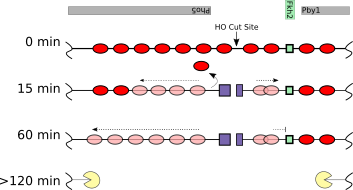
\includegraphics[width=2.5in]{r35_figures/cut_process.png}
\end{center}
\vspace{4mm}
\caption{DSB at the \textit{PHO5} locus. GCOP summary of the temporal dynamics of chromatin alterations immediately following a GAL::HO induced DSB at the \textit{PHO5} locus. }%
\end{floatingfigure}


%In collaboration with the Haber laboratory (Haber letter) we have used markerless CRISPR/Cas9\cite{Dekker2017} to introduce multiple ectopic HO-endonuclease recognition sequences into six loci with distinct chromatin states (TF bound regions, centromeres, telomeres, etc.) in a single GAL::HO yeast strain.  %Site specific DSBs at these ectopic loci is rapid and dependent on GAL::HO induction.% and is rapid with 90\% of the DNA being cut within 15-30 minutes of galactose addition.  
%We are able to %simultaneously 
%to comprehensively, and in a factor agnostic manner, 
%monitor the specific chromatin changes that occur in response to a DSB over time in the absence of a donor template for repair.  Proof of principle experiments at the \textit{PHO5} locus reveal the asymmetric eviction of a flanking nucleosome, sliding of distal nucleosomes until impeded by a neighboring Fkh2 bound site and the recruitment of a DNA binding factor to the break ({\color{dukeblue}\textbf{Figure 5}}).  Although we can detect a new occupancy footprint at either side of the  break, we do not know the identity of the factor -- it could represent the MRX complex, Ku proteins, or even HO endonuclease itself. Importantly, the wealth of existing molecular and genetic data regarding trans-acting factors involved in double strand break recognition and repair %, coupled with the `awesome power of yeast genetics', 
%will enable us to undertake a %systematic
%candidate based approach to identify the responsible factor(s).  By simultaneously interrogating the site specific chromatin changes that occur across a broad survey of different ectopic locations for the break, we will begin to be able to identify the rules by which the local chromatin structure influences DSB recognition and the kinetics of repair.



\ssheading{Interrogating chromatin structure following repair}
%Repair of the DNA break may occur through either HR via a homologous donor template or NHEJ.  
We are interested in understanding how epigenetic information is restored following repair of the break. %Although prior experiments have clearly shown a loss of nucleosome occupancy surrounding the break at the MAT locus and in mammalian cells, these have all lacked the precision to observe subtle changes in chromatin organization and are often confounded by strand resectioning.
For example, at \textit{PHO5} immediately following a break we observe eviction of a flanking nucleosome as well as more distal nucleosomes sliding away from the break; 
If we turn off HO-endonuclease and 
allow the cells to proceed through repair by NHEJ in the absence of a donor template %or in a \textit{rad51} mutant 
does the resulting chromatin recapitulate the organization prior to the break? Although prior experiments have shown that both replication independent and dependent chromatin assembly mechanisms contribute to restoring nucleosome occupancy\citep{Li2016-wg}
%\citep{Tsabar2015,Li2016} 
they have lacked the resolution to precisely and quantitatively describe nucleosome occupancy and the re-association of TFs.
% or were conducted at the \textit{MAT} locus which has inherently poorly positioned nucleosomes\citep{Weiss1998-lq}.  
%We will be able to precisely and quantitatively assess the contribution of both replication dependent and independent mechanisms using well characterized mutants of chromatin assembly pathways for the re-establishment of chromatin following repair at multiple locations each with unique chromatin states.
  
A more complicated challenge is to assess chromatin changes that occur during and after homology driven repair as %PCR and genomic-based approaches to study nucleosome occupancy lack the ability 
it is difficult to readily distinguish the donor sequence from the sequence-identical recipient. 
%Experiments at the mating type loci in yeast have begun to elucidate specific changes in chromatin structure\citep{Hicks2011-di,Tsabar2016-le}; however, the inherently poor nucleosome positioning at the \textit{MAT} locus\citep{Weiss1998-lq} and silenced nature of \textit{HML} and \textit{HMR} loci\citep{Rusche2003-wy} may not be representative of the rest of the genome.  
%revealed chromatin changes however 
%or were conducted at the \textit{MAT} locus which has inherently poorly positioned nucleosomes\citep{Weiss1998-lq}.
We propose to discriminate between the donor and the broken recipient by specifically labeling either sequence with the nucleoside analogue, EdU ({\color{dukeblue}\textbf{Figure 6}}). Sequences proximal ($<$15 kb) to early origins can be specifically labeled %to early   We and others have previously demonstrated that it is possible to specifically label only those sequences proximal ($<$15 kb) to early replicating origins, 
by releasing cells from a G1 $\alpha$-factor arrest into hydroxyurea (HU) in the presence of BrdU or EdU\citep{Peace2016-rb,Belsky2015-li}.  Importantly, these cells can be released back into the cell cycle and will retain the early origin-specific labeling for several generations.  We have engineered a yeast strain with an $\sim$4.5 kb duplication of the  \textit{PHO5} locus inserted adjacent to  \textit{ARS214} on the same chromosome.  Both copies of the \textit{PHO5} locus contain either an intact or mutant HO recognition site. Induction of a break in either the endogenous \textit{PHO5} locus or at the \textit{ARS214} proximal copy will allow us to specifically track the temporal progression of chromatin changes on either the donor or the break template.  Together these experiments will provide a base pair resolution view of the temporal kinetics of chromatin re-establishement and will likely provide critical insights into how epigenetic state is preserved or lost following a DNA damage.
\begin{floatingfigure}[l]{3.7in}
\vspace{-5mm}
\begin{center}
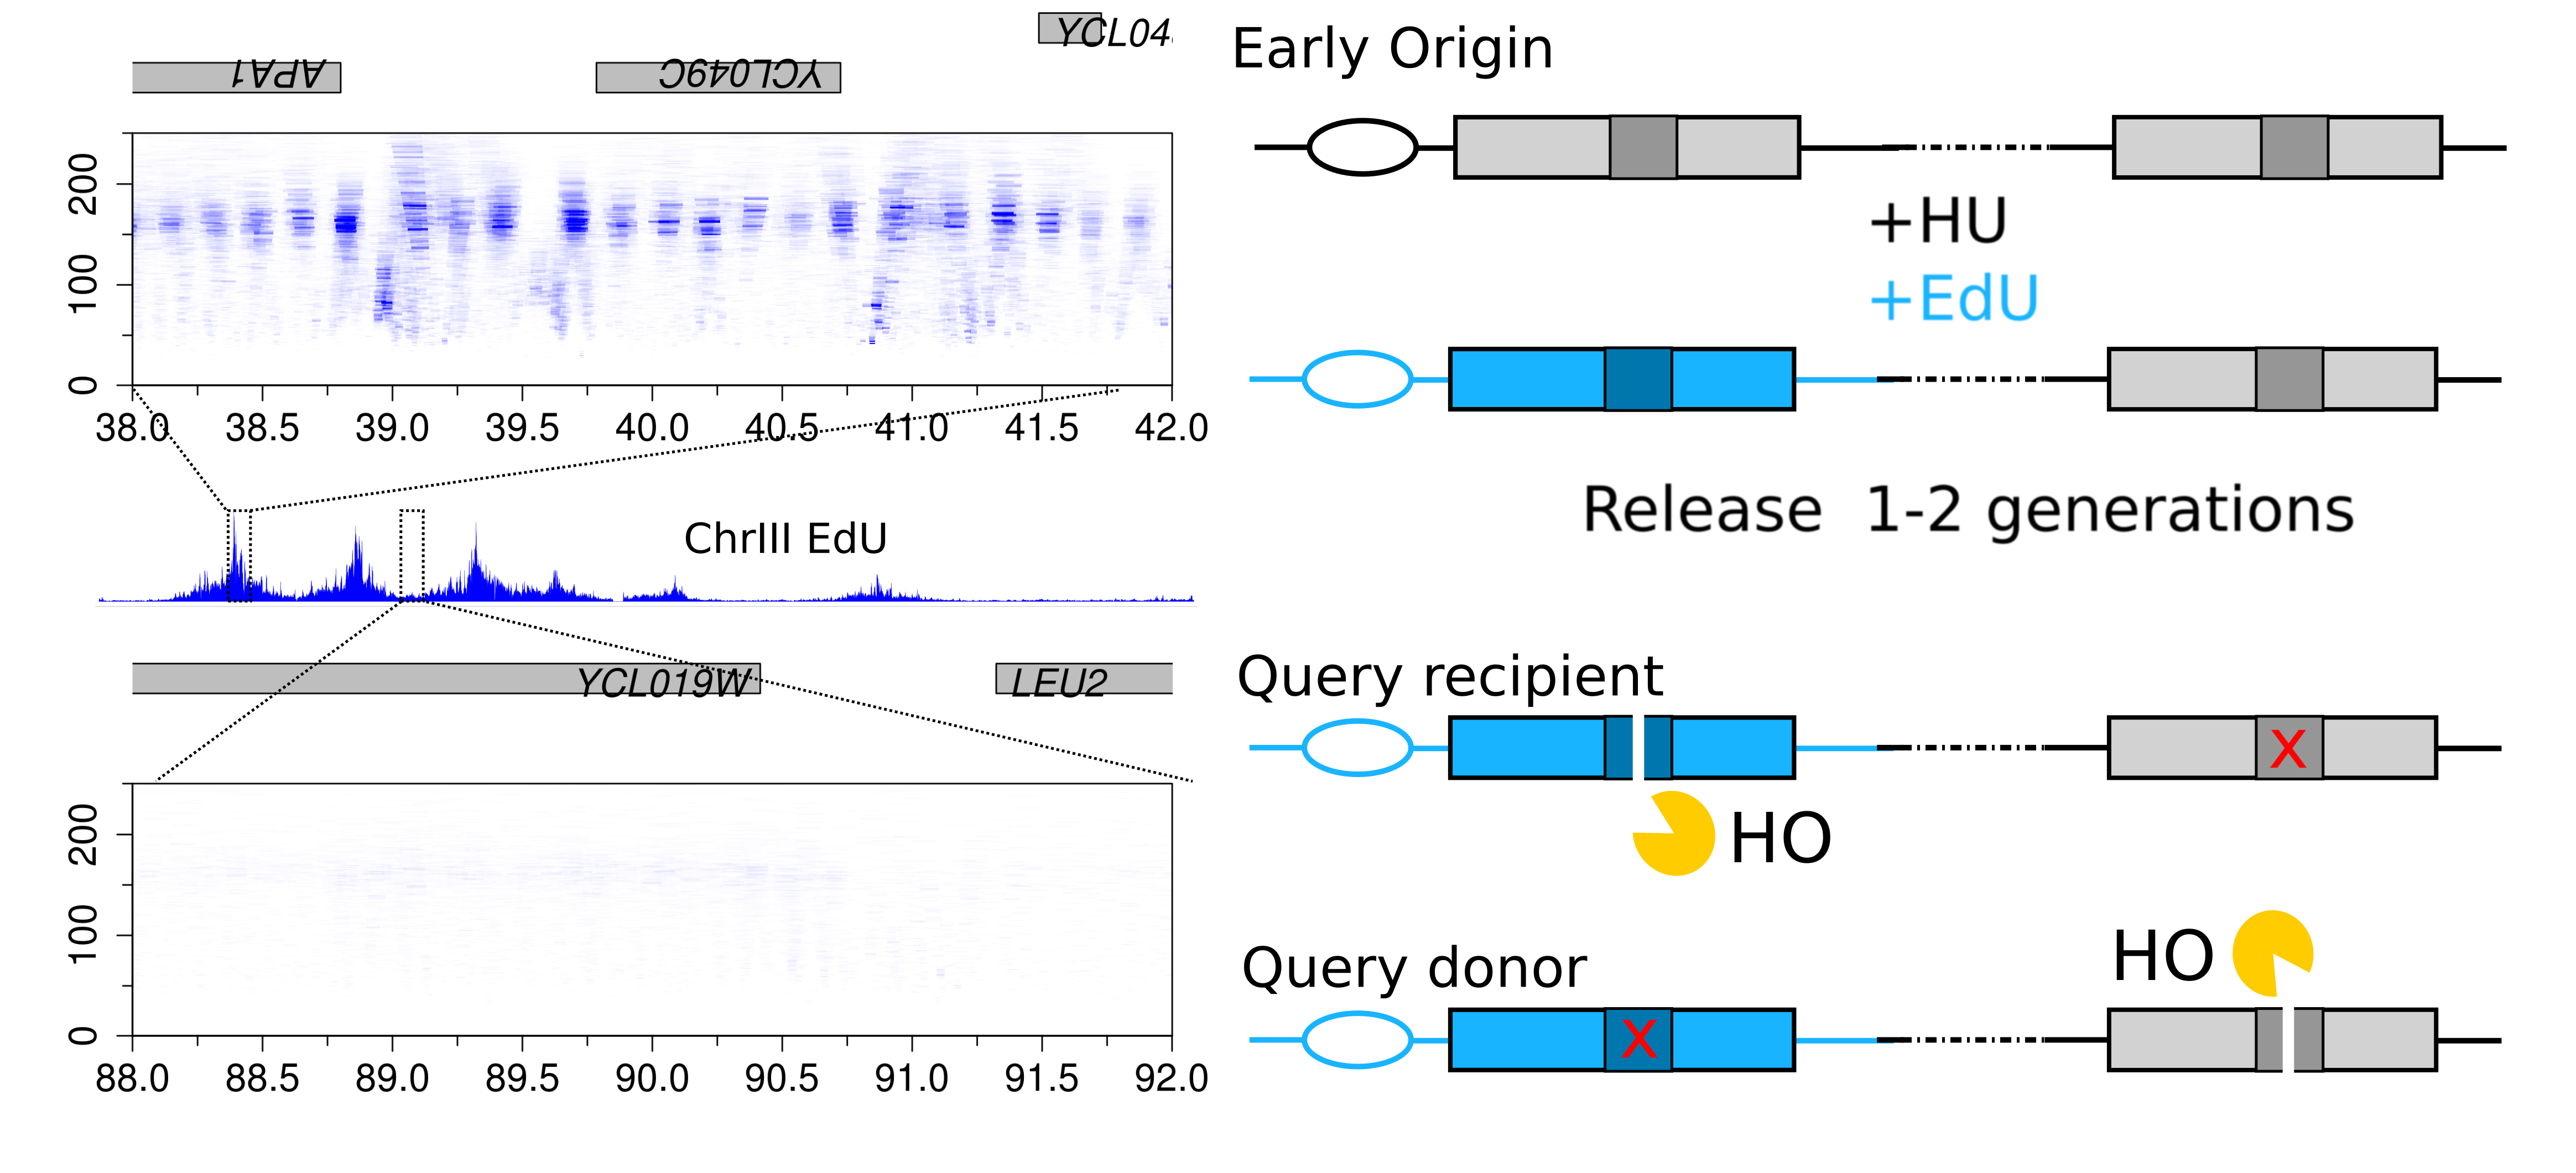
\includegraphics[width=3.7in]{r35_figures/edu_schematic_27.png}
\end{center}
\vspace{7mm}
\caption{Differentiating donor from recipient chromatin.  \textbf{Left}. EdU labeling early origin proximal chromatin structure.  \textbf{Right}.  Schematic for labeling either donor or recipient (damaged) DNA. }%
\end{floatingfigure}


%Importantly, both copies contain either an intact ectopic HO-endocuclease site or a 1 bp indel resistant to cleavage by HO-endonuclease.  Thus, we can induce a break in either the endogenous \texit{PHO5} locus or the identical \texit{ARS214} proximal copy which will enable us to specifically track the temporal progression of chromatin changes on either the donor or the break template.  Together these experiments will provide a nucleotide resolution view of the temporal kinetics of chromatin re-establishement and will likely provide critical insights into epigenetic state is preserved or lost following a DNA damage.

%siupstream of the \textit{PHO5} locus 

%We have engineered a yeast strain with an ectopic HO-endonuclease site upstream of \textit{PHO5} on chromosome II and ~4.5kb homologous donor sequence (containing a single 1bp indel resistant to cleavage by HO-endonuclease) that has been integrated adjacent to an early origin (\textit{ARS214} on the same chromosome.  

%Chromatin at the homologous donor template will be specifically labeled with EdU in the presence of HU and then released back into the cell cycle for at least one generation prior to generating the DSB.  Total chromatin will be digested with MNase to generate GCOPs. EdU specific GCOPs will be enriched by click chemistry-mediated biotinylation and streptavidin capture. We expect to identify donor specific perturbations of chromatin structure that are required to facilitate strand invasion and repair.

%nhej in G1 arrested cells. G2 will have donor



%In collaboration with Jim Haber (Brandeis; see letter of support) we have begun to elucidate the chromatin changes that occur 

%In order to repair a double strand break through HR, a search for a homologous donor sequence must be efficiently conducted across the genome.  Recent \invitro single molecule experiments with rad51 or recA pre-synaptic nucleoprotein filaments have begun to elucidate the mechanics of homology search on naked donor template DNA\cite{Renkawitz2014}.  However, a major question remains -- how is homology search conducted \invivo by the rad51 presynaptic filament in the context of chromatin? Recombination induced gene-conversion experiments have clearly demonstrated a dependence on chromatin remodelers such as INO80\cite{Tsukuda2009,Horigome2014}.  A major challenge to addressing this question using genome-wide approaches is the inability to readily distinguish homologous donor sequences from the sequence-identical damaged template DNA.   We propose to discriminate between the donor and break template by specifically labeling donor template with the nucleoside analogue, EdU ({\color{dukeblue}\textbf{Figure 6}}).   We and others have previously demonstrated that it is possible to specifically label only those sequences proximal ($<$15 kb) to early replicating origins, by releasing cells from a G1 alpha factor arrest into hydroxyurea (HU) in the presence of BrdU or EdU\citep{Peace2016-rb,Belsky2015-li}.  Importantly, these cells can be released back into the cell cycle for several generations and will retain the early origin-specific labeling albeit at diluted levels.  We have engineered a yeast strain with an ectopic HO-endonuclease site upstream of \textit{PHO5} on chromosome II and ~4.5kb homologous donor sequence (containing a single 1bp indel resistant to cleavage by HO-endonuclease) that has been integrated adjacent to an early (\textit{ARS214} or \textit{ARS305}) on the same or different chromosome.  Chromatin at the homologous donor template will be specifically labeled with EdU in the presence of HU and then released back into the cell cycle for at least one generation prior to generating the DSB.  Total chromatin will be digested with MNase to generate GCOPs.  EdU specific GCOPs will be enriched by click chemistry-mediated biotinylation and streptavidin capture. We expect to identify donor specific perturbations of chromatin structure that are required to facilitate strand invasion and repair.  Finally, we should be able to delay or repress specific remodeling events by the depletion or sequestration of key ATP-dependent chromatin remodelers (\eg Ino80).

%\newpage

\sheading{Transcription}
A major challenge in the post-genomic era is to understand how the information encoded in a static DNA sequence is capable of dynamic and regulated cell type specific patterns of gene expression. We are working in collaboration (R01 GM118551) with Alex Hartemink (PI) and Greg Crawford to develop predictive models of genome-wide transcript production from genome-wide chromatin occupancy data %({\color{dukeblue}\textbf{Figure 7}}). 
Specifically, robust statistical models are being developed and validated for predicting gene expression by simultaneously monitoring real-time chromatin occupancy and dynamic transcription rates as synchronized yeast cells progress through the cell cycle\citep{Orlando2008-jq}.  Importantly, the statistical framework and quantitative tools developed for this project will be also be applicable to the temporal dynamics of chromatin changes that occur during DNA replication and repair.
%\begin{floatingfigure}[l]{2.5in}
%\vspace{-5mm}
%\begin{center}
%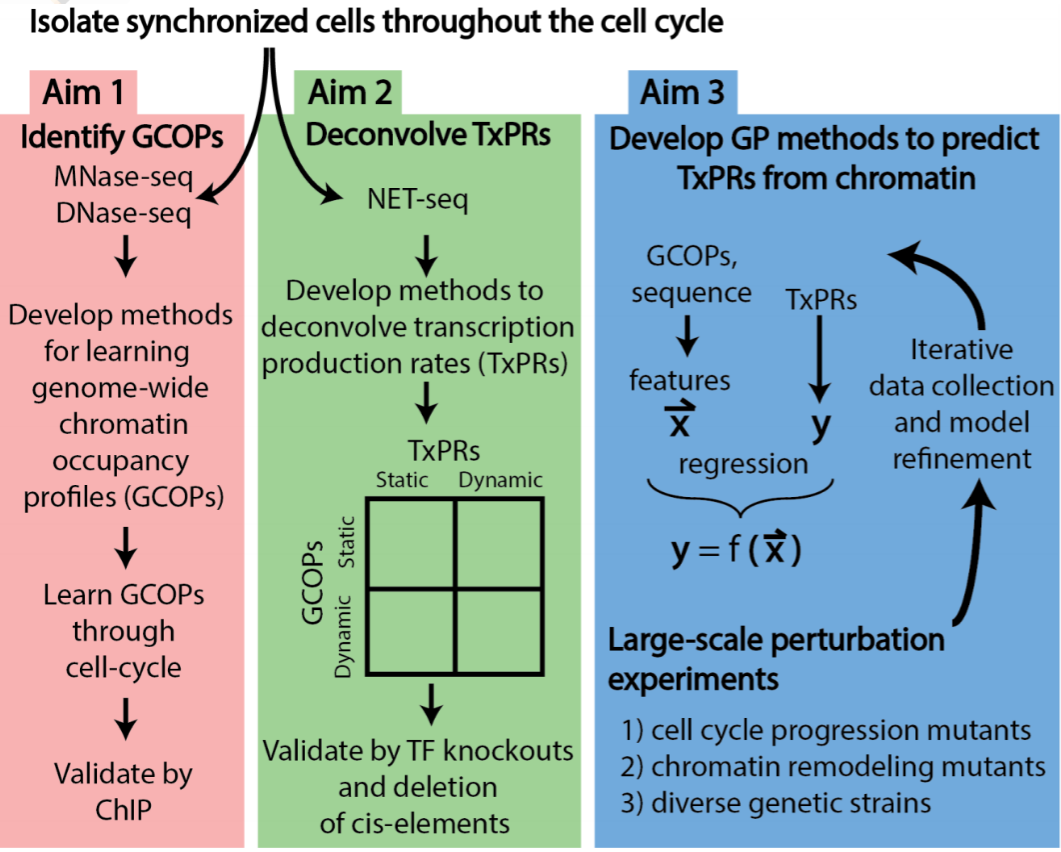
\includegraphics[width=2.5in]{r35_figures/gcop_strategy.png}
%\end{center}
%\vspace{2mm}
%\caption{Schematic describing the approach and methodologies to develop predictive models of cell cycle regulated gene expression from chromatin occupancy data. }%
%\end{floatingfigure}

My research program has benefited from the long standing collaboration we have had with the Hartemink group\citep{MacAlpine2010-ju,Belsky2015-li}.  Contributing to the success of the collaboration is the physical proximity of our research space in the Levine Science Research Center and mutual interest in cell cycle, DNA replication and chromatin structure.  We fully expect this productive collaboration to continue into the foreseeable future. 

\pagebreak
\bibliography{paperpile}


%Expected findings:
%-no change suggests homology search supports the model of querying donor strands while associated with histones on the outside
%- we will likely see a change since haber saw something in a locus adjacent to MATa (basically saw nucleosome depletion)
%Rad51 dependent changes suggest changes specific to homology search and not dsb
%Search from inside out or proximal edge? length of homology needed? where does search start.
%cis vs trans donor/break
%Extent of chromatin remodeling
%Impact of in80

%Recipriocal experiment -- Specially label cut site at ARS214 and/or ARS305 to rule out broader chromatin effects. but also query the chromatin changes that occur following repair of the break. how is broken chromatin reestablished.

%Epigenetic scar at donor or break

%Alternative approach -- also possible to do ChIP-seq for specific factors (eg. rad51) on EdU labeled chromatin. ORGANIC-ChIP + EdU (this is getting complicated but cool)




%they are thought to promote chromatin assembly and dissasembly at the replication fork.  

%their role at o

%MCM complex histone H3 interaction which 


%The Mcm2 subunit has been shown to directly interact with histone H3 presumably to faciliate chromatin disassembly and assembly ahead of the replication fork.  Work from our laboratory and rhind laboratory suggest that Mcm also appears to be in complex with nucleosome at the origin during G1.  




%We will test the impact of the mcm mutant on complex formation -- unlikey to be an intitation defect.  We will also take a proteomic approach to identify possible 



%Work in the Rhind laboratory has shown that chromatin immunoprecipitation of the MCM complex from MNase treated chromatin results in the recovery of nucleosomal sized DNA fragments\cite{}. 

%stochastic transcription termination.  

%Mcm2-7 has been previously shown to interact with histone H3 via ...  Although, this interaction is thought to mediate chromatin assembly via asf1, it may also be necessary for the observed Mcm2-7 nucleosome interaction at the origin.  We will test this hypothesis by performing ChIp-seq on mutant Mcm2-7. If the amino acid is required for nucleosome interaction, we will expect to lose the mcm-27+nucleosome chip-signal.  Could be shaped by nearby 3' transcription. To avoid torriosional consequences. knock out the promoter.



%We will 

%epigenetic angle -- specific modifications -- proteomic approach

%histone interaction domain?





%We will use a 

%Specific questions we hope to address include 

%Although


%Put another way -- at origin, we find the Mcm2-7 complex associated with either the up or down stream nucleosome.  Similar results were also identified by Nick Rhind and colleagues.  What is the molecular basis for this symmetry and nucleosome association? and how does it impact origin efficiency and timing. 



%How to identify factors that limit 1 mcm double hexamer per origin.  candidate approach.  multiple mcm loading -- stepwise during double hexamer loading...

%histone modifications?  topological constraints? why do both nucleosomes not become loaded?

%proteomic approach?  transcription and supercoiling?  examine netseq and supercoiling parameters during displacement via transcription?  Does transcription shape the effect? h3.3





%\sssheading{level 3} What does this look like. in the greater context.
%mcm loading -- asymmmetry. proteomic apprroach 

%factors that direct -- txp?

%Tie into in vitro experiments with Steve Bell.  We 
%The MacAlpine and Hartemink groups have had a long standing collaboration 

%This work will not only reveal how changes in chromatin occupancy are related to gene expression

%The proposed research will result in (i) efficient new methods for producing quantitative GCOPs that will be applicable in any organism with a sequenced genome; (ii) GCOPs from budding yeast as they progress through the cell cycle, revealing for the first time in any organism how genome-wide chromatin occupancy changes over the course of the cell cycle; (iii) characterization of how genome-wide chromatin changes are linked to changes in TxPRs, not only in wild-type yeast, but also under a wide range of genetic and genomic perturbations; and (iv) models learned from all these data that can predict TxPRs on the basis of chromatin occupancy, providing mechanistic insight into how the cell-cycle–regulated transcription program is influenced by its changing chromatin state. The DNA sequence of the genome is static, yet the dynamics in chromatin state and transcription rates can  Importantly, this project will allow us to look into the black box of chromatin Cell cycle -- This work will overtake our commitment with Hartemink laboratory to characterize big picture question of cell cycle regulation look inside black box. 



%Though the genome’s sequence is essentially fixed, its state may be constantly changing inside a cell. Two aspects of this changing state are the specific arrangement of myriad protein complexes along the genome in the form of chromatin, and the current rate of transcript production for each gene. A fundamental research objective is to understand the relationship between these two, and in particular, how transcript production rates (TxPRs) are influenced by genome-wide chromatin state. The goal of this proposal is to develop models that are capable of predicting a cell’s genome-wide transcription state from knowledge of its genome-wide chromatin state. To build such models requires simultaneously profiling a cell’s genome-wide chromatin state and transcription state at different times or under different conditions: Observing how the two change together, particularly in the context of directed perturbation, provides the statistical leverage needed to build predictive models that can provide causal insight. In this proposal, models will be developed and validated by monitoring chromatin and transcription in budding yeast as they progress through the cell cycle, a temporal series of highly regulated events controlling cell proliferation, aberrations of which can lead to cancer. Owing to the complexity of this challenge, yeast is used as a starting point because of its compact genome and genetic tractability, but we anticipate our methods will also be applicable in more complex organisms, including human. One major obstacle is that state-of-the-art chromatin immunoprecipitation (ChIP) methods for assaying chromatin state require a separate experiment not only for each time point and experimental condition, but also for each of the 100s–1000s of types of proteins binding along the genome. To overcome this hurdle, this proposal describes a novel method for efficiently learning quantitative genome-wide chromatin occupancy profiles (GCOPs) using nuclease-digested chromatin at single-base resolution. The proposed method enables the comprehensive determination of quantitative chromatin occupancy of transcription factors, nucleosomes, and other DNA-binding factors across the entire genome without requiring a separate experiment for each. Producing GCOPs in conjunction with high resolution measurements of TxPRs will allow the development of sophisticated, mechanistically interpretable models that predict transcript production rates as a function of chromatin state.

%The proposed research will result in (i) efficient new methods for producing quantitative GCOPs that will be applicable in any organism with a sequenced genome; (ii) GCOPs from budding yeast as they progress through the cell cycle, revealing for the first time in any organism how genome-wide chromatin occupancy changes over the course of the cell cycle; (iii) characterization of how genome-wide chromatin changes are linked to changes in TxPRs, not only in wild-type yeast, but also under a wide range of genetic and genomic perturbations; and (iv) models learned from all these data that can predict TxPRs on the basis of chromatin occupancy, providing mechanistic insight into how the cell-cycle–regulated transcription program is influenced by its changing chromatin state. The DNA sequence of the genome is static, yet the dynamics in chromatin state and transcription rates can  Importnatly, this project will allow us to look into the black box of chromatin Cell cycle -- This work will overtake our commitment with Hartemink laboratory to characterize big picture question of cell cycle regulation look inside black box. 